\section{Kommunikation}

Das Kommunikationskonzept stellt die Grundlage für die reibungslose Verständigung der Teammitglieder dar und regelt die Kommunikation mit dem Auftraggeber. Das Sitzungsprotokoll wird abwechselnd von einem Teammitglied geschrieben. Die Strukturierung des Kommunikationskonzept ist in der folgenden Abbildung \ref{fig::Kommunikationskonzept} ersichtlich.

\begin{figure}[h] 
\centering
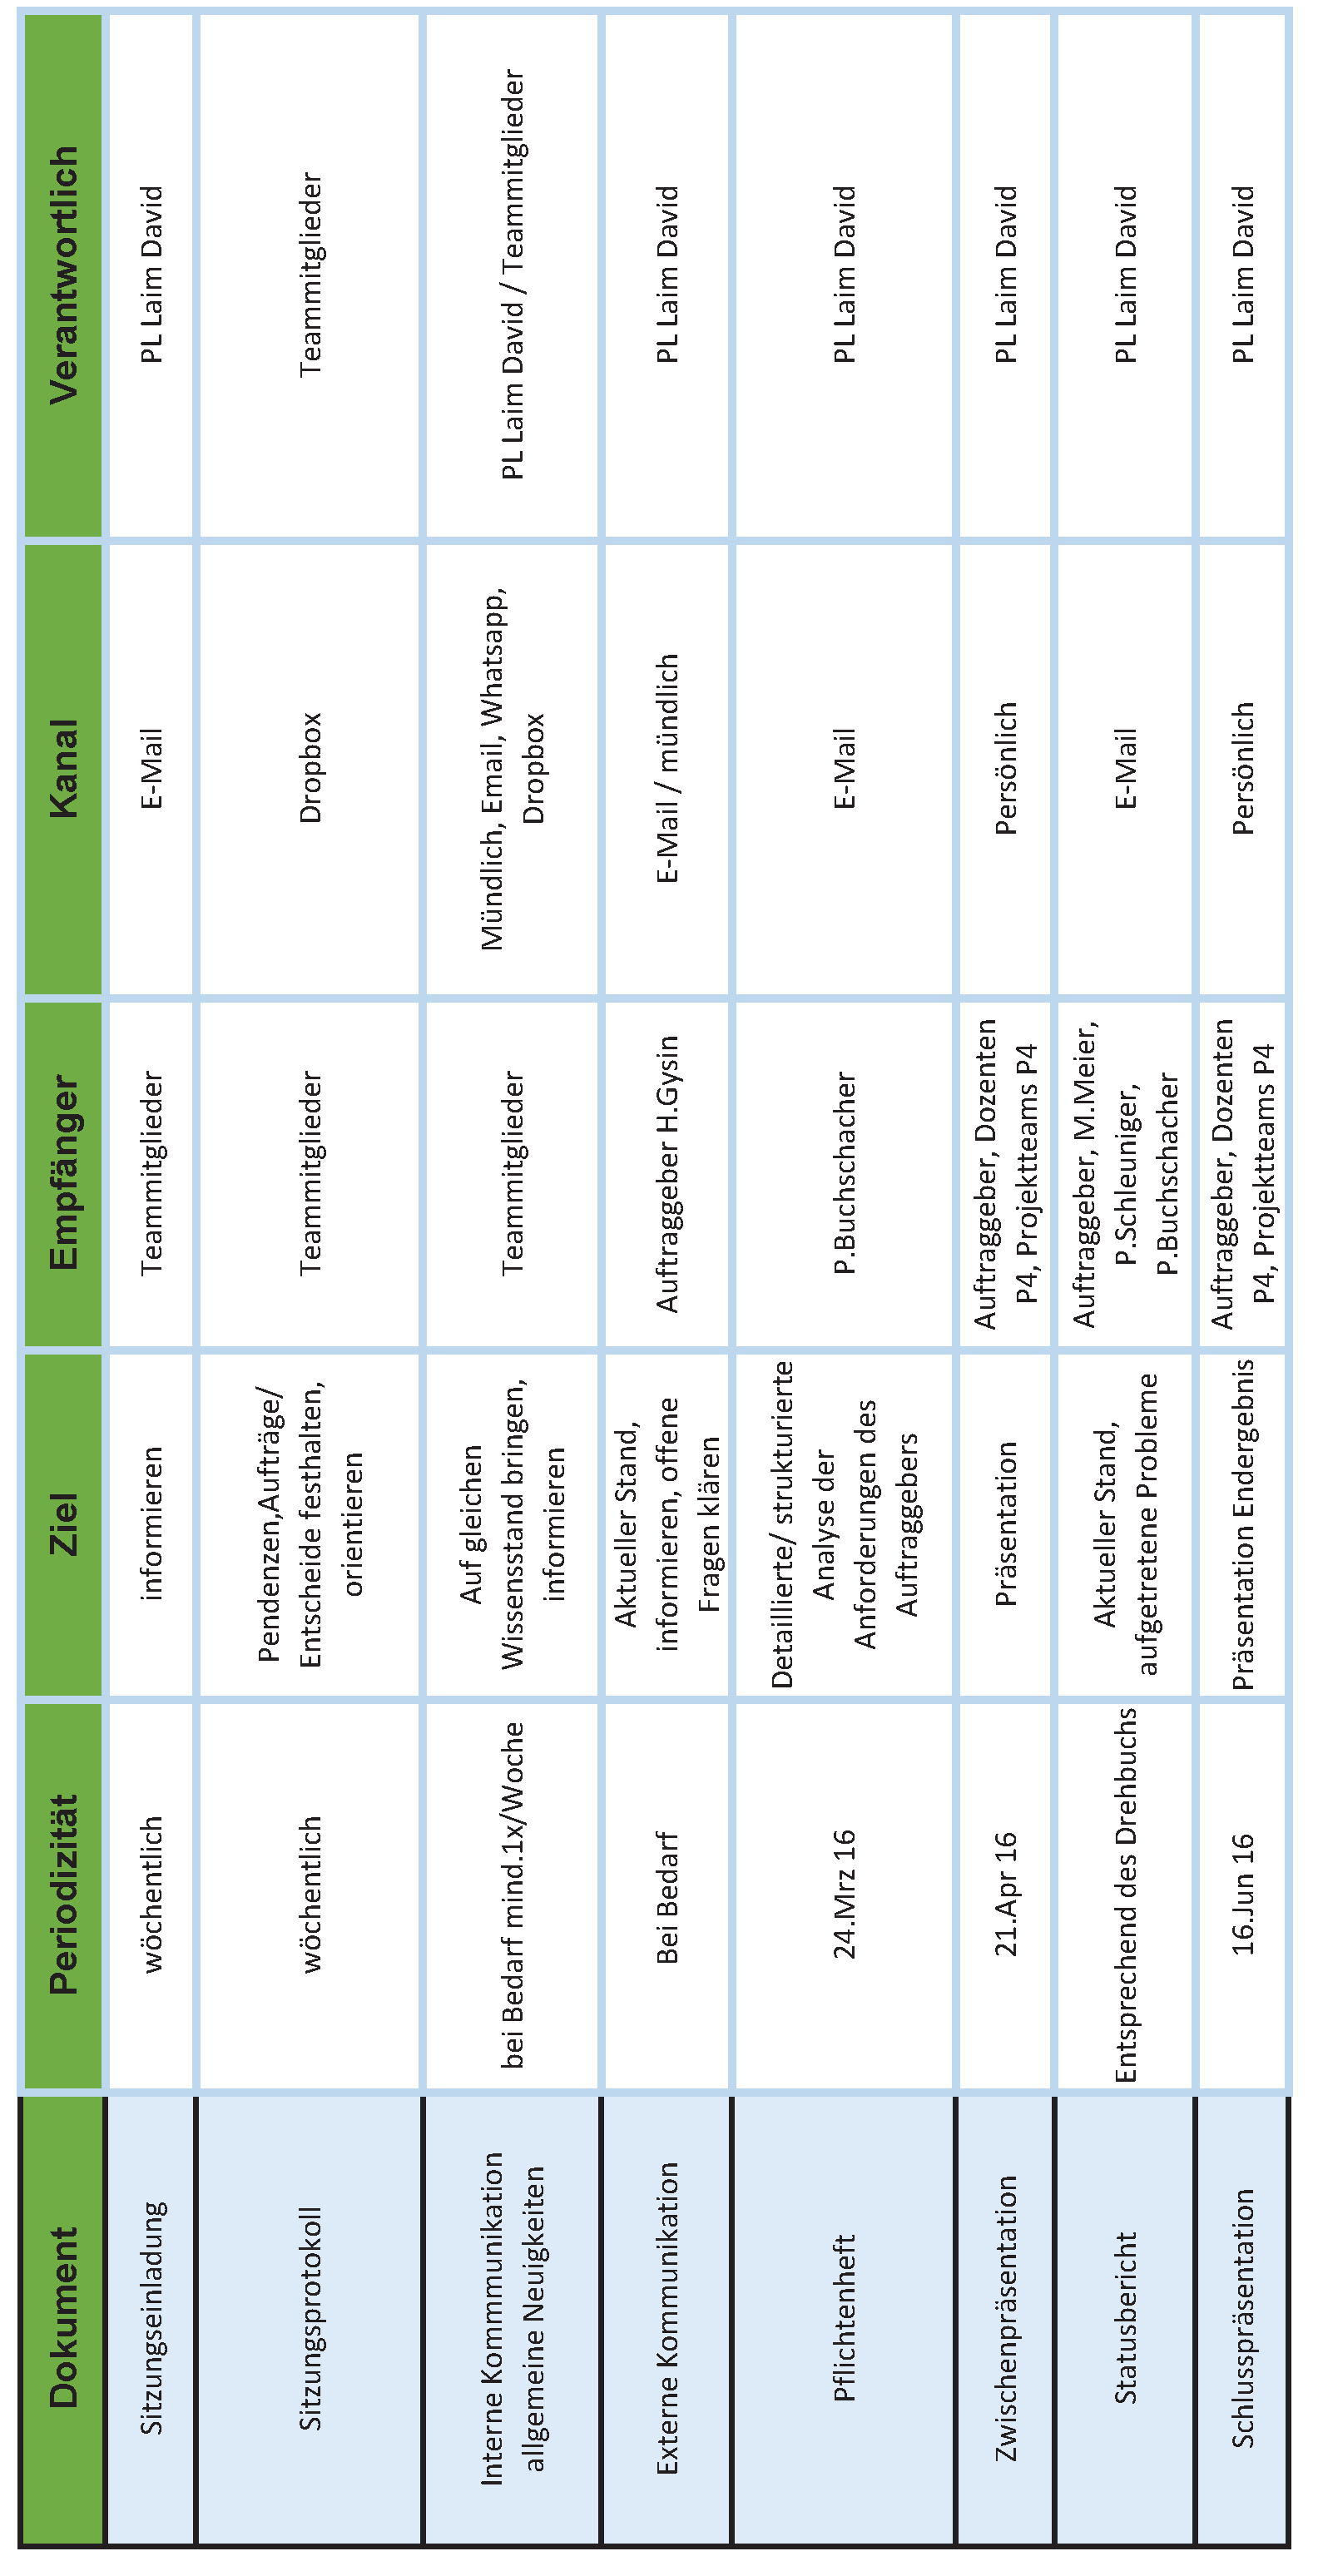
\includegraphics[width=0.55\textwidth]{Kommunikationskonzept.png}%
\caption{Kommunikationskonzept}%
\label{fig::Kommunikationskonzept}%
\end{figure}